
\chapter{Modèle de chargement}
\label{ch:loading-model}

Un système est composé d'un ensemble d'éléments (modules) qui interagissent
entre eux. L'interaction entre les module est dans un contexte statique ou
dynamique. Dans le contexte statique les modules sont incorporés au sein de
l'application. Dans le contexte dynamique les modules sont externe à
l'application.

\section{Chargement des bibliothèques}

%La collection des modules s'effectue au sein d'un

% TODO: voir chargé
Le chargement d'une bibliothèque Scheme (ou module) dans Gambit est séparé en
plusieurs niveaux. Il y a la phase recherche du module et de ces dépendances
qui valide la présence de toutes les modules nécessaire.  Ensuite le module et
ses dépendances sont chargés dans un ordre qui suit les relations de
dépendance.  Un module est soit sur le disque ou déjà en mémoire.
L'emplacement des bibliothèques sur le système de fichier est lié par défaut
aux chemin spécifié par le \lstinline{##module-search-order} a comme défaut
\lstinline{~~lib} et \lstinline{~~userlib}.

La procédure exacte de chargement des bibliothèques par \verb|import| n'est pas
spécifier par le standard R7RS. Le standard spécifie seulement une syntaxe de
base et le de comportement principal qui est requis. L'importation d'une
bibliothèque doit chargé la bibliothèque et rendre c'est fonctionnalité
disponible dans le contexte l'importation a eu lieu qui peut soit ovenir d'un
programme principale ou d'une bibliothèque.

Le chargement d'une bibliothèque peut-être effectuée à l'exécution par
l'utilisation de \texttt{eval} (par \texttt{load}) pour les fichiers source et
\texttt{load-object-file} pour les bibliothèques compilées. Cette recherche
peut aussi avoir lieu durant l'édition des lien en utilisant les méta-infos
contenus dans les \textbf{.c} qui sont chacun compilé par le compilateur C
en \textbf{.o} et lié par le \textit{linker}.
\section{Modèle statique}

Le modèle de bibliothèque statique consiste à intégrer la bibliothèques
dans l'application finale. La bibliothèque n'a pas besoin d'être chargé
durant l'exécution. L'avantage du modèle statique est le déploiement.
Puisque tout les dépendances sont dans l'application finale¸ il suffit
de distribué celle-ci. Le compilateur Gambit support un modèle statique
pour des programme simple. Compiler un application lié statiquement est
possible de façon manuelle. Pour lié statiquement deux fichiers Scheme
simple il suffit d'invoquer le \texttt{gsc} comme suit:

\begin{center}
  \lstset{language={Scheme}}
\begin{mplisting}{0.4}
  $ gsc file1.scm file2.scm
\end{mplisting}
\end{center}

% Par la contrainte des systèmes, le premier type de bibliothèques utilisé
% étaient dit statique.  Elles consistaient en un regroupement logique de
% plusieurs fichiers objets en un archive (.a). La création d'une bibliothèque
% statique peut s'effectuer avec l'utilitaire \verb|ar|. Lorsque que programme se
% lie à une bibliothèque statique, il inclut tout simplement l'ensemble des
% procédures contenu dans les fichiers objets. L'avantage des bibliothèques
% statiques est de regrouper plusieurs fonctionnalité commune en un seul concept,
% par exemple la bibliothèque mathématique \verb|libm.a| qui contient les
% fonctions mathématique (i.e. \verb|cos|, \verb|sin|).  En plus,  fait que le
% processus d'édition des liens, qui consiste à associer les noms des
% fonctionnalités avec leur valeur (AMBIGU), n'est effectué juste une fois. Une
% liaison avec une bibliothèque statique \verb|libfoo.a| qui contient le fichier
% objet \verb|foo.o| est équivalent à une liaison directe avec le fichier
% \verb|foo.o|.

% \begin{figure}[ht]
%     \begin{minipage}[t]{0.5\textwidth}
% \begin{verbatim}
% # Création de la bibliothèque statique libfoo.a
% ar rcs libfoo.a foo.o
% # Création de l'exécutable main.exe
% ld -o main.exe main.o libfoo.a
% \end{verbatim}
%     \end{minipage}
%     \caption{Exemple de création de bibliothèque statique suivit d'un exemple
%     d'utilisation.}
% \end{figure}

% \todo{Citation}

Un des problèmes du modèle statique est le coût lié à la maintenance.  Les
programmes qui utilise des bibliothèques statiques ne permettent pas une
construction modulaire. La mise à niveau d'une des bibliothèques statiques
nécessite la recompilation du programme au complet. En plus, cela n'est pas
adapté pour des applications évolutifs qui peuvent être étendu
par l'utilisateur. Une solution qui a été adopté est le
modèle dynamique~\ref{sec:ch4_model_dynamic}. Cela offre une plus grande
liberté dans la conception des programmes.


\section{Modèle dynamique}
\label{sec:ch4_model_dynamic}

Dans le modèle dynamique chaque module est séparé durant l'exécution.
L'application contient les informations pour extraire les fonctionnalités des
modules durant l'exécution. Le déploiement d'un application nécessite la
distribution de toutes les dépendance.  Les bibliothèques partagés offre
plusieurs avantages par rapport aux bibliothèques statique.

Dans ce modèle les bibliothèques sont lié au programme durant l'exécution. Cela
nécessite que les bibliothèques soit organisé sur le système de fichier d'une façon
distinguable. Chaque module doit posséder un nom unique qui permet d'y référer.
Ce nom unique va être utilisé lors de la collection des dépendances.


%Les bibliothèques
%sont soit en code source ou compilé nativement avec l'extension (\textit{.oN})
%où le N correspond à la version du binaire qui commence à 1.


La recherche des bibliothèques est effectué dans un ordre spécifique
indépendant de la spécification.  L'algorithme de recherche les bibliothèques
prend entré le nom de la bibliothèque et retourne le chemin absolu
correspondant à sont emplacement dans l'arborescence du système de fichier. Les
bibliothèques sont situées dans différents répertoires l'origine du programme,
le répertoire des bibliothèques système (\lstinline{~~lib}) et le
répertoire de bibliothèque utilisateur (\lstinline{~~userlib}).

% \begin{itemize}
%   %% XXX: directory where the executable is located (usefull for devel no need to install the module). collecté
%   \item \verb|origin/dummy.sld|
%   \item \verb|origin/dummy/dummy.sld|
%   \item \verb|~~userlib/dummy.sld|
%   \item \verb|~~userlib/dummy/dummy.sld|
%   \item \verb|~~lib/dummy.sld|
%   \item \verb|~~lib/dummy/dummy.sld|
% \end{itemize}

Chaque module possède trois niveaux d'initialisation dans le système numérotés de
0 à 2. Le niveau 0 indique que le module est collecté, mais non initialisé. Le
niveau 1 indique que le descripteur du module à été récupéré. Le niveau 2 marque
les module chargé qui sont près à être utilisé.

Soit un système avec les dépendance suivante:
\begin{figure}[ht]
  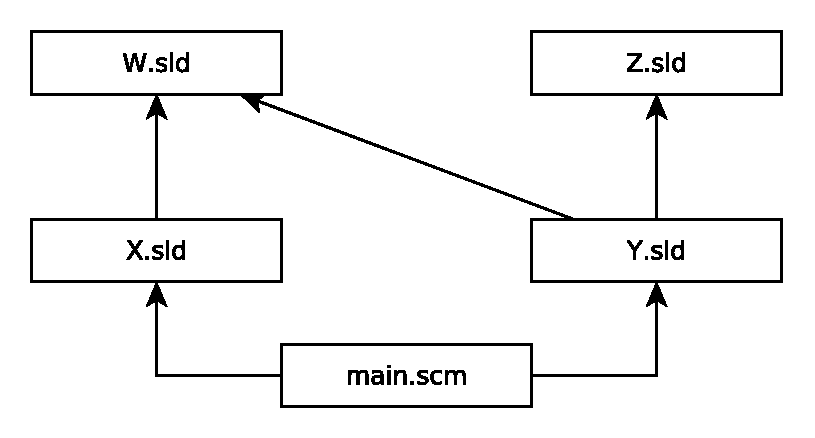
\includegraphics{figures/system-example}
  \caption{Un exemple d'un système fictif composé de différents modules.
  Le module principale se nomme \textbf{main.scm} avec l'extension \textbf{.scm}
  et les bibliothèques ont l'extension \textbf{.sld}}
\end{figure} % TODO: use yed for that graph


Le démarrage du module principal \textbf{main.scm} déclenche la collection des
modules X et Y, qui récursivement déclenche la collection de W et Z.
L'algorithme de collection des modules gère les modules qui apparaisse
plusieurs fois au sein du graphe.  Une fois la collection de tous ces modules
est complété le descripteur de module est récupéré par un appels aux primitives
du système d'exploitation si compilé.


\section{Module hébergé}

Un module qui est hébergé est un module qui dont son contenu
se retrouve sur un domaine comme \url{github.com}. La syntaxe
des noms de domaine est inspiré du RFC-2396.
La différence avec la spécification du \textit{hostname} dans le RFC-2396
est que le \textit{hostname} ne peut pas finir par un point et doit contenir
au moins un \verb|domainlabel|. C'est pour permettre de distingué
un module local et un module hébergé. \\

\begin{center}
  \lstset{caption={Grammaire BNF représentant un hostname selon un sous
  ensemble du RFC-2396.},captionpos=b,frame=single}
  \begin{mplisting}{0.9}
hostname      = +( domainlabel "." ) toplabel
domainlabel   = alphanum | alphanum *( alphanum | "-" ) alphanum
toplabel      = alpha | alpha *( alphanum | "-" ) alphanum
alphanum      = alpha | digit
alpha         = [a-zA-Z]
digit         = [0-9]
\end{mplisting}
  \label{lst:hostname->grammar}
\end{center}


\subsection{Installation automatique}
L'installation automatique d'un module dépend du contenu de la \textit{whitelist}.
La \textit{whitelist} contient une liste de préfixe de \textit{<module-ref>}.

Un module hébergé est installé automatiquement s'il est présent dans la liste
nommée \textit{whitelist}. Cette contient des préfixes de \textit{<module-ref>}
qui sont considéré par l'utilisateur de confiance. Par défaut \texttt{github.com/gambit}
est inclus dans cette liste.  Cela implique que tous les modules sous \texttt{github.com/gambit}
peuvent être installé automatiquement.


\begin{center}
  \begin{mplisting}{0.4}
$ gsi -:whitelist=github.com/foo
> (##os-module-whitelist)
("github.com/gambit" "github.com/foo")
\end{mplisting}
\end{center}

%L'installation d'un module hébergé dont le no


\subsection{Module \texttt{\_git}}

Ce module offre un interface pour utiliser interagir avec les des dépôts git.
Il permet de cloner un dépôts qui est hébergé sur \url{github.com}. Un clone du
dépôts est simplement un copie qui contient les informations suffisantes pour
passer d'une version d'un module à un autre. L'opération qui permet de changer
de version est \emph{checkout}.


%-------------------------------------------------------------------------------
%
%Modèle "link dynamique" :
%  recherche des libs au run time, utilisation de eval (par load) et
%  load-object-file
%
%  % gsi main.scm      ou      % gsc main.scm ; gsi main.o1
%
%    origin/main.scm    : (import X Y)
%          /X/X.sld     : (import)
%
% ~~userlib/Y/Y.sld     : (import Z)
%
%     ~~lib/Z/Z.sld     : (import)
%          /Z.o1
%
%-------------------------------------------------------------------------------
%
%Modèle "link statique" :
%  recherche des libs au link time en utilisant les méta-infos
%  dans les .c (demand-lib et supply-lib), chaque .c compilé en
%  un .o séparément et les .o linkés par le compilateur C
%
%  % gsc -obj -keep-c X.sld      ;; créer .c et .o
%  % gsc -obj -keep-c Y.sld      ;; créer .c et .o
%  % gsc -obj -keep-c Z.sld      ;; créer .c et .o
%  % gsc -obj -keep-c main.scm   ;; créer .c et .o
%  % gsc -exe main.c             ;; combine les .o pour créer main.exe
%
%    origin/main.scm    : (import X Y)
%          /main.c      : (demand-lib X Y)
%          /main.o
%          /X/X.sld     : (import)
%            /X.c       : (demand-lib) (supply-lib X)
%            /X.o
%
% ~~userlib/Y/Y.sld     : (import Z)
%          /Y/Y.c       : (demand-lib Z) (supply-lib Y)
%          /Y/Y.o
%
%     ~~lib/Z/Z.sld     : (import)
%          /Z/Z.c       : (demand-lib) (supply-lib Z)
%          /Z/Z.o
%
%-------------------------------------------------------------------------------
%
%Modèle "whole-program" :
%  recherche des libs au compile time en utilisant les imports
%  dans les fichiers sources, les AST de toutes les libs fusionnées
%  en un seul AST compilé par gsc (donc un seul .c généré et compilé
%  par le compilateur C pour créer main.exe)
%
%  % gsc -exe -whole-program main.scm
%
%    origin/main.scm    : (import X Y)
%          /X/X.sld     : (import)
%
% ~~userlib/Y/Y.sld     : (import Z)
%
%     ~~lib/Z/Z.sld     : (import)
%
%-------------------------------------------------------------------------------
% correction d’une petite coquille…
% /Y.c       : (demand-lib Z) (supply-lib Y)
% /Y.o
%
% ~~lib/Z/Z.sld     : (import)
% /Z.c       : (demand-lib) (supply-lib Z)
% ...


% (check-sld "/tmp/scheme/base/base.sld" "/tmp/scheme/base")
% (check-sld "/tmp/scheme/base.sld" "/tmp/scheme")
% (check-sld
%  "/home/frederic/Documents/MasterResearch/gambit9/lib/cocolappin/scheme/base/base.sld"
%  "/home/frederic/Documents/MasterResearch/gambit9/lib/cocolappin/scheme/base")
% (check-sld
%  "/home/frederic/Documents/MasterResearch/gambit9/lib/cocolappin/scheme/base.sld"
%  "/home/frederic/Documents/MasterResearch/gambit9/lib/cocolappin/scheme")
% (check-sld
%  "/home/frederic/Documents/MasterResearch/g9/lib/scheme/base/base.sld"
%  "/home/frederic/Documents/MasterResearch/g9/lib/scheme/base")
% object-file-path: /home/frederic/Documents/MasterResearch/g9/lib/scheme/base/.gambit_409003@C/base.o1
% ("/home/frederic/Documents/MasterResearch/g9/lib/scheme/base/base.sld"
%  .
%  #<input-port #2 "/home/frederic/Documents/MasterResearch/g9/lib/scheme/base/base.sld">)
